
\chapter{\uppercase{The Moment-Based Low-Order Equations}}

The formation of the LO equations is similar to a discontinuous FE method.  Weighted
integrals of the the equations are taken with functions that have local support as weight
functions.  The equations are written with element-wise moments of $I$ and $T$ as
unknowns.  Leaving the solution in this form allows for use of information form a
previous HO solution to eliminate auxillary unknowns from the equations. This is different than a standard Galerkin FE
method~\cite{fe_book} where a
functional form of the solution is directly assumed. The final equations will have a
similar form to S$_2$ equations, but we have not used a collocation method in angle,
which should limit ray effects~\cite{ray_effects} in higher spatial dimensions.
The equations eliminate extra spatial unknowns in a manner similar to to a linear-discontinuous FE
method~\cite{morel_ldtrt}.  We also explore the
possibility of using the MC solution to modify the discretization of the LO solution in
Sec.~\ref{sec:spat_clos}.   MOVE


The remainder of this chapter is structured as follows: the general moments will be
derived and then the angular and spatial closure are discussed REWRITE.  For
simplicity, the implicit Euler discretization is used throughout this section.
Sec.~\ref{sec:time_cont} will use the HO solution and MC transport to consistently
close the equations in time, improving time accuracy.

\section{Forming the Space-Angle Moment Equations}

\subsection{LO Spatial mesh and Finite-Element Spatial Moments}

The LO equations are formulated over a FE mesh.  The domain for the $i$-th spatial
element (or cell) has support $x\in[x_{i-1/2},x_{i+1/2}]$ with width $h_i=x_{i+1/2} -
x_\il$ and cell center 
$x_i = x_\il + h_i/2$.  There is a total of $N_c$ elements, spanning the
spatial domain $0\leq x\leq X$.  For simplicity, this spatial mesh is fixed throughout the
simulation.  Mesh adaptation is only applied in the HO solver.

\begin{figure}[H]
    \centering
    \begin{centering}
        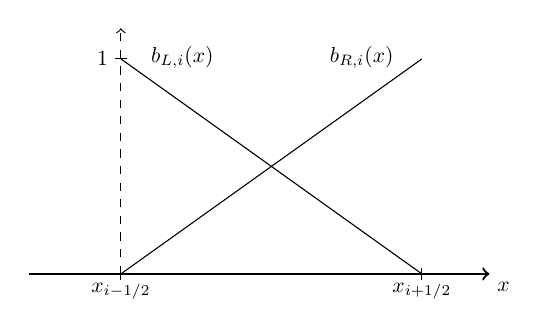
\begin{tikzpicture}[scale=0.78, every node/.style={transform shape}]
            \node at (10.7,4.0) {${1}$  };
            \draw (10.9,4.0) -- (11.1,4.0);
            \draw (11.0,0.4) -- (11.0,0.6) node[below, pos=0.4] {$x_{i-1/2}$};
            \draw (15.90,0.4) -- (15.90,0.6) node[below, pos=0.4] {$x_{i+1/2}$};
            \node at (14.92,4.02) {$b_{R,i}(x)$};
            \node at (12.0,4.02) {$b_{L,i}(x)$};
            \draw [thick,->] (9.5,0.5) -- (17.0,0.5) node[anchor=north west] {$x$};
            \draw [dashed,->] (11.0,0.5) -- (11.0,4.5);
            \draw (11.0,0.5) -- (15.90,4.0);
            \draw (15.90,0.5) -- (11.0,4.0);
        \end{tikzpicture}
    \end{centering}
    \caption{Illustration of linear finite element basis functions $b_{L,i}(x)$ and
    $b_{R,i}(x)$ for spatial element $i$.\label{fig:lin_fe}}
\end{figure}

The spatial moments are defined by integrals weighted with the standard linear finite element (FE)
interpolatory basis functions.  An illustration of the two linear FE basis functions for the $i$-th element is
given in Fig.~\ref{fig:lin_fe}.  The left basis function is defined as
\begin{equation}
    b_{L,i}(x)= \left\{\begin{matrix} \frac{x_\ir - x}{h_i} & x_\il \leq x \leq x_\ir
        \\ 0 &  \text{elsewhere}
    \end{matrix}\right.,
\end{equation}
corresponding to the node $x_\il$.
The right basis function is 
\begin{equation}
    b_{R,i}(x)= \left\{\begin{matrix} \frac{x - x_\il}{h_i} & x_\il \leq x \leq x_\ir
        \\ 0 & \text{elsewhere}
    \end{matrix}\right. ,
\end{equation}
corresponding to the node $x_\ir$. With these definitions, a local linear approximation to a
function $f$ can be formulated as $f(x)\simeq f_{L,i} b_{L,i}(x) + f_{R,i}
b_{R,i}(x),\quad x\in[x_{\il},x_{\ir}]$.\footnote{In literature the FE functions are
formally defined with support over two adjacent elements.  However, in our notation our 
functions only have non-zero support in element $i$. This accommodates our later
definition of moments and discontinuous unknowns.}

The spatial moments are defined by integrals over the each element, using the two
basis functions.  We use $\mom{\cdot}$ to indicate integration over a
spatial element.  The spatial moments are
\begin{equation}\label{eq:x_moml}
\mom{\cdot}_{L,i} = \frac{2}{h_i} \int_{x_{i-1/2}}^{\xr} b_{L,i}(x) (\cdot) \dd x
\end{equation}
and
\begin{equation}\label{eq:x_momr}
\mom{\cdot}_{R,i} = \frac{2}{h_i} \int_{x_{i-1/2}}^{\xr} b_{R,i}(x) (\cdot) \dd x.
\end{equation}
where the factor of $2/h_i$ is a normalization constant.
It is noted in this notation $\mom{\phi}_{L,i}$ and
$\mom{\phi}_{R,i}$ represent spatial moments of the intensity over cell $i$, opposed
to $\phi_{L,i}$ and $\phi_{R,i}$, which represent the interior value of the linear
representation of $\phi(x)$ at $x_\il$ and $x_\ir$ within the cell. 

To simplify notation and discussion, we also define the slope and average moments over a
spatial cell.  The average scalar intensity is
\begin{equation}
    \phi_i = \frac{1}{h_i} \int_{\xl}^{\xr} \phi(x) \dd x
\end{equation}
and
\begin{equation}
    \phi_{x,i} = \frac{6}{h_i} \int_{\xl}^{\xr} \left(\frac{x-x_i}{h_i} \right)
    \phi(x) \dd x . 
\end{equation}
The linear representation over a cell in terms of these moments is $\phi(x) = \phi_i
+ 2/h_{i}^2 \phi_x (x - x_i)$, for $x\in(\xl,\xr)$. 

\subsection{Definition of Angular Moments}

To reduce the angular dimensionality, positive and
negative half-range integrals of the angular intensity are taken.  The half-range
integrals of $I$ are defined as $ \phi^+(x) = 2 \pi \int_0^{1} I(x,\mu)\, \dd \mu$ and $
\phi^-(x) = 2 \pi \int_{-1}^{0} I(x,\mu) \,\dd
\mu$, respectively.  Thus, in terms of half-range quantities, the mean intensity is $\phi(x) = \phi^-(x) +
\phi ^+(x)$.

\subsection{Space-Angle Moments of the Transport Equation}

The LO radiation equations are formed by applying the space and angle moment operators to the
transport equation and performing algebraic manipulation.  We provide a detailed
derivation of the $L$ and $+$ radiation equation, and state the final results for the
other moment operators.  First, the $L$ moment operator is applied to the time-discretized transport equation,
i.e., Eq.~\eqref{eq:trans_td}.  Integration by parts on the streaming term yields
\begin{multline}\label{eq:spat_mom}
    -2{\mu}_{i-1/2} I_{i-1/2}^{n+1} + \frac{2}{h_i}\int_{\xl}^{\xr} \mu I^{n+1} \dd x
        +  \left(\sigma_{t,i}^{n+1}+\frac{1}{c \Delta t} \right) h_i 
  \mom{\phi}_{L,i}^{n+1,+} \\-  \frac{\sigma_{s,i} h_i}{2} \left( \mom{\phi}_{L,i}^{n+1,+} +
  \mom\phi_{L,i}^{n+1,-}\right) = \frac{h_i}{2} \mom{\sigma_a^{n+1} a c T^{n+1,4}}_{L,i} +
  \frac{h_i}{c\Delta t}\mom{\phi}_{L,i}^{n,+}.
\end{multline}
Here, the cross sections have been assumed constant over a cell.  The mean
intensity in the scattering term is expanded in terms of half-range unknowns.
REWRITE: ADD USEFUL RELATIONS BETWEEN THE MOMENTS TO THE APPENDIX
Additionally, the relation in Eq.~\eqref{eq:LtoA} is used to eliminate the integral from the
equation is terms of $L$ and $R$ moments:
\begin{multline}\label{eq:spat_mom}
    -2{\mu}_{i-1/2} I_{i-1/2}^{n+1} + \mom{\mu I^{n+1}}_{L,i} + \mom{\mu I^{n+1}}_{R,i} 
        +  \left(\sigma_{t,i}^{n+1}+\frac{1}{c \Delta t} \right) h_i 
  \mom{\phi}_{L,i}^{n+1,+} \\-  \frac{\sigma_{s,i} h_i}{2} \left( \mom{\phi}_{L,i}^{n+1,+} +
  \mom\phi_{L,i}^{n+1,-}\right) = \frac{h_i}{2} \mom{\sigma_a^{n+1} a c T^{n+1,4}}_{L,i} +
  \frac{h_i}{c\Delta t}\mom{\phi}_{L,i}^{n,+}.
\end{multline}

The resulting equation is integrated over the positive half range:












\subsection{Radiation Energy Equations}

Pairwise application of the $L$ and $R$ basis
moments with the $+$ and $-$ half-range integrals to Eq.~\eqref{ho_trans} 
ultimately yields four moment
equations per cell. As in~\cite{wolters}, algebraic manipulation is performed to form
intensity-weighted
averages of $\mu$, which we denote as consistency terms.  As an example, the equation resulting from application of the $L$ moment and
positive half-range integral is
\begin{multline}\label{eq:lo_tran}
    -2{\mu}_{i-1/2}^{n+1,+} \phi_{i-1/2}^{n+1,+} + \cur {\mu}_{L,i}^{n+1,+}
  \mom{\phi}_{L,i}^{n+1,+}
  +  \cur\mu_{R,i}^{n+1,+}
  \mom{\phi}_{R,i}^{n+1,+} +  \left(\sigma_{t,i}^{n+1}+\frac{1}{c \Delta t} \right) h_i 
  \mom{\phi}_{L,i}^{n+1,+} \\-  \frac{\sigma_{s,i} h_i}{2} \left( \mom{\phi}_{L,i}^{n+1,+} +
  \mom\phi_{L,i}^{n+1,-}\right) = \frac{h_i}{2} \mom{\sigma_a^{n+1} a c T^{n+1,4}}_{L,i} +
  \frac{h_i}{c\Delta t}\mom{\phi}_{L,i}^{n,+},
\end{multline}
where the $\phi^+_{i-1/2}$ and $\mu^+_{i-1/2}$ terms represent face-averaged quantities at $x_{\il}$.  The negative direction and $R$ moment equations are
derived analogously.  The element-averaged angular consistency terms are defined in terms of half-range integrals, e.g.,
\begin{equation}\label{const}
    \cur{{\mu}}_{L,i}^{n+1,+} \equiv \frac{\mom{\mu I^{n+1}}_{L,i}^+}{\mom{I^{n+1}}_{L,i}^+} =  \frac{
{\displaystyle \frac{2}{h_i}} \int\limits_0^1 \int\limits_\xl^\xr \mu \, b_{L,i}(x)
I^{n+1}(x,\mu) \dd x \dd \mu } 
{{\displaystyle \frac{2}{h_i}} \int\limits_0^1 \int\limits_\xl^\xr \, b_{L,i}(x)
I^{n+1}(x,\mu) \dd x \dd \mu } .
\end{equation}
The $\mu_{i-1/2}^{n+1,+}$ term is defined analogously and represents an angular average on the face at $x_{\il}$.

\subsection{Material Energy Equations}

To derive the LO material energy equations, $T(x)$ is represented spatially in
the LDFE trial space, i.e.,
$ T(x) \simeq T_{L,i} b_{L,i}(x) + T_{R,i} b_{R,i}(x),\quad x\in(x_{i-1/2},x_\ir)$.
Similarly, the emission term is represented in the material and radiation equations with the LDFE
interpolant $T^4(x)\simeq T_{L,i}^4 b_{L,i}(x) + T_{R,i}^4 b_{R,i}(x)$.   The $L$ and $R$ spatial moments are taken of the material
energy equations; the LDFE representations for $T(x)$ and $\sigma_a a c T^4(x)$ are used to
simplify the spatial integrals. For example, the final LO material energy
 equation resulting from application of the $L$ moment is
 \begin{multline}\label{lo_mat_dis}
     \frac{\rho_i c_{v,i}}{\Delta t}\left[ \left(\frac{2}{3}T_{L,i} + \frac{1}{3}T_{R,i}
        \right)^{n+1} - \left(\frac{2}{3}T_{L,i} + \frac{1}{3}T_{R,i}
    \right)^{n} \right]  + \sigma_{a,i}^{n+1} \left( \mom{\phi}_{L,i}^+ +
    \mom{\phi}_{L,i}^- \right)^{n+1} \\ = \sigma_{a,i}^{n+1}a c
\left( \frac{2}{3} T_{L,i}^4 + \frac{1}{3}T_{R,i}^4
        \right)^{n+1}.
\end{multline}
Cross sections have been assumed constant over each element, evaluated at the
average temperature within the element, i.e., $\sigma_{a,i}^{n+1} =
\sigma_{a,i}([T^{n+1}_{L,i}+T^{n+1}_{R,i}]/2)$.
Because the material energy balance
 only contains angularly integrated quantities, there is no need to take angular
 moments of the above equation.  

\section{Closing the System with Information from the HO solution}
\label{sec:closure}

The six degrees of freedom (DOF) over each cell $i$ are the four moments $\mom{\phi}_{L,i}^+$,
$\mom{\phi}_{R,i}^+$, $\mom{\phi}_{L,i}^-$, and $\mom{\phi}_{R,i}^-$ and the two
spatial edge values $T_{L,i}$ and $T_{R,i}$. The four radiation and two material
energy equations define a system of equations for the six DOF, coupled to other cells
via upwinding in the streaming term.
The relation between the volume and face averaged quantities and the angular consistency parameters (e.g., Eq.~\eqref{const}) are not known a priori. 
A lagged estimate of $I^{n+1}$ from the previous HO solve is
used to estimate the angular consistency parameters. In the HOLO algorithm, the equations for LO unknowns at iteration $k+1$ use consistency parameters
computed (via relations, e.g., Eq.~\eqref{const}) using the latest HO solution $\tilde{I}^{n+1,k+1/2}$
as an approximation for $I^{n+1}(x,\mu)$. To close the LO system spatially, a linear-discontinuous (LD) spatial closure with the usual upwinding
approximation is used.  For example, for positive flow (e.g., Eq.~\eqref{eq:lo_tran}) the face terms $\mu_{i-1/2}$ and $\phi_{i-1/2}$
are upwinded from the previous cell $i-1$ or from a boundary condition; the terms
at $x_{i+1/2}$ are linearly extrapolated, computed using the $L$ and $R$ basis
moments, e.g., $\phi^+_{i+1/2} = 2\mom{\phi}_R^+ - \mom{\phi}_L^+$. 
Because there are no derivatives of $T$ in Eq.~\eqref{lo_mat}, there is no need
to define $T$ on the faces; the temperature has been assumed linear within a cell to
relate $T$ and $T^4$.  

The choice of a LD spatial closure should preserve the equilibrium diffusion limit.  In this limit, the MC HO solution will estimate angular consistency terms 
associated with an isotropic intensity, based on a spatially LD emission source.  The isotropic-intensity consistency terms will produce
LO equations that are equivalent to $S_2$ equations, with quadrature points of $\pm 1/2$.  Because the spatial
closure produces equations that are equivalent to an LDFE solution to these equations, we expect the equations to preserve the
equilibrium diffusion limit~\cite{morel_newton,densmore_edl}.

The linear-discontinuous (LD) closure with upwinding is not strictly positive.  In particular, for
optically thick cells with a steep intensity gradient, the solution becomes negative.
These negative values of intensity can propagate to adjacent cells. In thick regions of
TRT problems, reasonably fine spatial cells can still be on the order of millions of mean
free paths; negative values with an LD representation are unavoidable in practice for
such cells and mesh refinement is of minimal use.  Typically, for a standard LDFE method,
the equations are lumped to produce a strictly positive solution (for 1D)~\cite{morel_newton}. However, standard FE lumping
procedures would introduce difficulties in computing the consistency terms from the
HO solution.  Thus, an alternative spatial closure is used that is equivalent to the
standard FE lumping procedure.  The $L$ and $R$ moments are defined the same as before,
preserving the average within a cell, but the relation between the moments and
the outflow is modified.   For example, for positive $\mu$,
the outflow is now defined as $\phi^+_{i+1/2} = \mom{\phi}_R^+.$  Because the basis function $b_{R,i}(x)$ is strictly
positive, the outflow is positive.  This closure is only used
in cells where negative intensities occur.

\subsection{Newton's Method for LO Equations}

Adding the equations for each cell together forms a global system of coupled equations.
The equations are nonlinear due to the Planckian emission source.  
We have used Newton's method to solve the nonlinear system, based on a typical linearization of the Planckian source with cross
sections evaluated at temperatures from the previous iteration, as described in~\cite{morel_newton}.  
Because we have only considered problems with constant densities and heat capacities, the
linearization described below is in terms of temperature $T$ rather than material internal
energy, for simplicity. However, the linearization can be formed in terms of internal energy
to apply this method to a general equation of state.

To formulate the Newton iterations, the Planckian source is linearized in the material and radiation equations (Eq.~\eqref{??}
\& Eq.~\eqref{???}). Application of the first order Taylor expansion in time to the
implicit emission source $B(T^{n+1})$, about some temperature $T^*$ at some
time $t^*\in[t^{n},t^{n+1}]$, yields
\begin{equation}\label{new_planck}
    \sigma_a^{n+1} a c T^{4,n+1} \simeq \sigma_a^* a c \left[T^{*4} + (T^{n+1} - T^*) 4T^{*3} \right]
\end{equation}
where $\sigma_a^*\equiv\sigma_a(T^*)$.  Substitution of this expression into Eq.~\eqref{eq:mat_cont} yields
\begin{equation}
    \rho c_v \left( \frac{T^{n+1} - T^{n}}{\Delta t} \right) = \sigma_a^* \phi^{n+1} -
    \sigma_a^* a c \left[ T^{*4} +  (T^{n+1} - T^*) 4T^{*3} \right].
\end{equation}
Algebraic manipulation of this equation yields an expression for $T^{n+1} - T^{*}$:
\begin{align*}
\left( T^{n+1} - T^* \right) &= \frac{ {\displaystyle \frac{\sigma_a^* \Delta t}{\rho
c_v}}  \left[ \phi^{n+1} -  a c T^{*4} \right] + (T^n - T^*) }{1 +
        \sigma_a^* a c \Delta t\frac{\displaystyle 4
T^{*3}}{\displaystyle \rho c_v } }.
\end{align*}
%This provides an expression for $T^{n+1}$ as a
%function of $T^*$ and the mean intensity $\phi^{n+1}$, i.e.,
%\begin{equation}
%\label{lo_t_new}
%T^{n+1}  = \frac{1}{\rho c_v } f\sigma_a^* \Delta t \left( \phi^{n+1} - c a T^{*4} \right)
%+ f T^n + (1-f) T^*.
%\end{equation}
This expression is substituted back into Eq.~\eqref{new_planck} to form
an explicit approximation for the emission source at $t^{n+1}$ as
\begin{equation}\label{t_next1}
    \sigma_a a c T^{4,n+1} \simeq \sigma_a^* (1 -f^*) \phi^{n+1}
    + f^* \sigma_a^* a c T^{4,n} + \rho c_v\frac{1-f^*}{\Delta t} (T^n - T^*)
\end{equation}
where $f^* = [1 + \sigma_a^* c \Delta t 4 a T^{*3}/(\rho c_v)]^{-1}$ is often referred to
as the Fleck factor~\cite{fnc}. 

Next, the above equation must be spatially discretized.  Application of the $L$ spatial
moment yields
\begin{multline}\label{eq:temp_const}
    \mom{\sigma_a^* a c T^{4,n+1}}_{L,i} = \sigma^*_{ai}(1-f_i^*)\mom{\phi^{n+1}}_{L,i} +
    f_i^*
    \sigma^*_{ai} a c \left(\frac{2}{3} T_{L,i}^{4,n} + \frac{1}{3} T_{R,i}^{4,n}\right)
    \\ \rho_i c_{vi} \frac{1 - f^*_i}{\Delta t} \left[\frac{2}{3}\left(T^n_{L,i} -
        T^*_{L,i}\right) + \frac{1}{3}\left(T^n_{R,i} -
    T^*_{R,i}\right)\right],
\end{multline}
where $T^{4,n}$ and $T^{n}$ have been assumed LD and $f^*$ is assumed constant over a cell, i.e., $f^*_i
\equiv \sigma_a(T_i^*)$.
The error introduced by a constant $f^*$ approaches zero as the
non-linearity is converged because $T^*$ approaches $T^{n+1}$. 
Based on an estimate for $T^*$, Eq.~\eqref{eq:temp_const} is an expression for
the Planckian emission source in the radiation moment equations with an additional effective scattering source.
A similar expression can be derived for $\mom{\sigma_{a,i} a c T^4}_R$ and the right
moment equations.
The expressions for the emissions source is substituted into the radiation moment equations
(Eq.~\eqref{eq:lo_tran}--~\eqref{???}) to produce a
linear system of equations for the new radiation intensity moments. 

Once the linear equations have been solved for new radiation moments, new temperature
unknowns can be estimated.  To conserve energy, the same linearization and discretizations used to
solve the radiation equation must be used in the material energy equation.
Substitution of Eq.~\eqref{eq:temp_const} into the material energy $L$ moment equation
ultimately yields
\begin{multline}\label{eq:new_temp}
    \frac{2}{3}T_{L,i}^{n+1} + \frac{1}{3}T_{R,i}^{n+1}= \frac{f_i^* \sigma_{ai}^* \Delta
t}{\rho c_{v}}  \left[ \mom{\phi^{n+1}}_{L,i}  - a c\left(\frac{2}{3} T_{L,i}^{4,n} + \frac{1}{3} T_{R,i}^{4,n}\right)
\right] + \\ (1- f^*_{i})\left(\frac{2}{3}T^*_{L,i} + \frac{1}{3}T^*_{R,i}\right) + f
\left(\frac{2}{3}T^n_{L,i} + \frac{1}{3}T^n_{R,i}\right)
\end{multline}
A similar expression is produced for the $R$ moment equation.  This produces a local
matrix equation to solve for new $T$ unknowns.  If both the radiation and temperature unknowns
are lumped, this matrix becomes diagonalized.

Based on these equations, the algorithm for solving the LO equations, with iteration index
$l$, is defined as
\begin{enumerate}
    \item Initialize $T$ unknowns using $T^n$ or the last estimate of $T^{n+1}$ from
        previous LO solve
    \item  Build the LO system based on the effective scattering $(1-f^l)$ and emission terms
          evaluated using $T^l$.
    \item Solve the linearized LO system to produce an estimate for $\phi^{n+1,l}$.
    \item Evaluate a new estimate of $T^{n+1}$ unknowns using Eq.~\eqref{eq:new_temp}.
    \item $T^*\leftarrow\tilde{T}^{n+1}$.
    \item Repeat 2-5 until $(T^{n+1,k})^4$ and $\phi^{n+1,k}$ are converged.
\end{enumerate}

\subsection{Direct Solution of the LO Equations}

Isotropic scattering,
including effective scattering terms from the linearization, are included in the system matrix. The system
matrix is an asymmetric, banded matrix with a band width of seven and is inverted
directly. 
Newton iterations are repeated until $\phi^{n+1}(x)$ and $T^{n+1}(x)$ are converged
to a desired relative tolerance.  Convergence is calculated using the spatial $L_2$
norm of the change in $\phi^{n+1}(x)$ and $T^{n+1}(x)$, relative to the norm of each
solution.  The lumping-equivalent discretization
discussed above is used for cells where the solution for
$\phi^{n+1}$ becomes negative. When negative values for $\phi^{n+1,\pm}(x)$ are detected, the lumping-equivalent discretization is used within
those cells and that Newton step is repeated. 


%Application of the first order Taylor expansion in time of the
%gray emission source, about some temperature $T^*$ at some
%time near $t^{n+1}$ gives
%\begin{equation}\label{new_planck}
%    \sigma_a^* a c T^{4,n+1} \simeq \sigma_a^* a c \left[T^{*4} + (T^{n+1} - T^*) 4T^{*3} \right]
%\end{equation}
%where the superscript $*$ denotes evaluation at $T^*$. A spatially discretized form
%of this expression is substituted
%into the emission term in the discretized material
%energy equations, e.g., Eq.~\eqref{lo_mat_dis}.  This allows for the material energy
%equation to be eliminated from the system, introducing effective scattering and
%emission sources into the right hand side
%of the LO radiation equations. This defines four linear equations for the four remaining radiation unknowns. 
%Once these linear equations have been solved for $\phi^{n+1}$, a new estimate of
%$T^{n+1}$ can be determined using the same linearization (Eq.~\eqref{new_planck}) to
%conserve the total energy.  This estimate of $T^{n+1}$ can now be used as $T^*$ to form a more
%accurate linearization of the emission source. 
